\documentclass[12pt]{article}

\usepackage{amsmath}
\usepackage{graphicx}
\usepackage{dcolumn}
\usepackage{booktabs}
\usepackage{rotating}

\usepackage{setspace}
\usepackage{parskip}
\usepackage[top=1in,bottom=1in,left=1in,right=1in]{geometry}

\usepackage{natbib}
\usepackage[pdfstartpage=1,pdfpagemode=UseNone,pdfstartview=FitH,pdffitwindow=true,bookmarks=false,colorlinks=true,linkcolor=blue,citecolor=blue]{hyperref}

% define lightgray
\usepackage[table]{xcolor}
\definecolor{lightgray}{gray}{0.9}

\begin{document}


%%%%%%%%%%%%%%%%%%%%%%%%%%%%%%%%
% Tables
%%%%%%%%%%%%%%%%%%%%%%%%%%%%%%%%
\clearpage
\section{Tables}

\begin{table}[!h]
    \caption{Sample filter steps}
    \centering
    \resizebox{\textwidth}{!}{\begin{tabular}{l>{\raggedright\arraybackslash}p{4in}ll}
   \toprule 
 
\multicolumn{4}{l}{{\bf Panel A:} Sample selection criteria} \\ 

&  & 
\multicolumn{2}{l}{Total (all countries)}
\\  
 
 
\multicolumn{1}{l}{Step} & 
\multicolumn{1}{l}{Description} 
& n & $\Delta$
\\ 
\cmidrule(lr){1-2}
\cmidrule(lr){3-4}
\\[-1.8ex]  
 
0 & Raw data & 415,771 &  \\ 
  1 & Panel years between 2000 and 2018 & 367,032 & -12\% \\ 
  2 & Prime age (25 - 54) & 210,900 & -43\% \\ 
  3 & Labour force participant (employed or unemployed) & 157,370 & -25\% \\ 
  4 & Non missing education or gender & 155,535 & -1\% \\ 
  5 & Hourly wages within the top/bottom 0.005 percentile & 154,743 & -1\% \\ 
  6 & Sample A: At least 3 observations & 79,148 & -49\% \\ 
  7 & Sample B: + always employed & 73,189 & -8\% \\ 
   
\hline \\[-1.8ex]  
 
\multicolumn{4}{l}{{\bf Panel B:} Data sets by event type} \\ 

& & 
\# & \%
\\ 
\cmidrule(lr){1-2}
\cmidrule(lr){3-4}
\\[-1.8ex]  
 
A & Unmp $\rightarrow$ perm & 3,670 & 5\% \\ 
  A & Unmp $\rightarrow$ temp & 1,268 & 2\% \\ 
  B & Temp $\rightarrow$ perm & 9,063 & 12\% \\ 
  B & Perm $\rightarrow$ temp & 6,800 & 9\% \\ 
   \bottomrule \\[-1.8ex] \multicolumn{4}{p{6in}}{Note: n - is unique observations.  $\Delta$ - is difference in n from previous step.  \# - is unique n who experienced at least 1 event.  \% - is percent who experienced an event.} 
\end{tabular}
}
    \label{table_sample_filter_steps}
\end{table}

\begin{table}[!h]
    \caption{Methodological simulation exercise}
    \begin{center}
    \resizebox{\textwidth}{!}{
\begin{tabular}{l c c c c c c c c c}
\toprule
 & \multicolumn{3}{c}{Simulation 1} & \multicolumn{3}{c}{Simulation 2} & \multicolumn{3}{c}{Simulation 3} \\
\cmidrule(lr){2-4} \cmidrule(lr){5-7} \cmidrule(lr){8-10}
 & FE & FEIS & AFE + DIF & FE & FEIS & AFE + DIF & FE & FEIS & AFE + DIF \\
\midrule
Temp                     & $-30.00^{***}$ & $-30.00^{***}$ &          & $-60.00$  & $-30.00^{***}$ &          & $-5.00$   & $-5.00$   &          \\
                         & $(0.00)$       & $(0.00)$       &          & $(31.46)$ & $(0.00)$       &          & $(26.22)$ & $(27.64)$ &          \\
Event: T $\rightarrow$ P &                &                & $30.00$  &           &                & $50.00$  &           &           & $30.00$  \\
                         &                &                & $(0.00)$ &           &                & $(0.00)$ &           &           & $(0.00)$ \\
Event: P $\rightarrow$ T &                &                & $-30.00$ &           &                & $-30.00$ &           &           & $20.00$  \\
                         &                &                & $(0.00)$ &           &                & $(0.00)$ &           &           & $(0.00)$ \\
\bottomrule
\multicolumn{10}{l}{\scriptsize{$^{***}p<0.001$; $^{**}p<0.01$; $^{*}p<0.05$. Note: In AFE + DIF, pre and post event coefficients are not shown.}}
\end{tabular}
}
    \label{table_simulation}
    \end{center}
\end{table}

%%%%%%%%%%%%%%%%%%%%%%%%%%%%%%%%
% Graphs
%%%%%%%%%%%%%%%%%%%%%%%%%%%%%%%%
\clearpage
\section{Graphs}

\begin{sidewaysfigure}[h!]
    \caption{Methodological simulation exercise}
    \resizebox{\textwidth}{!}{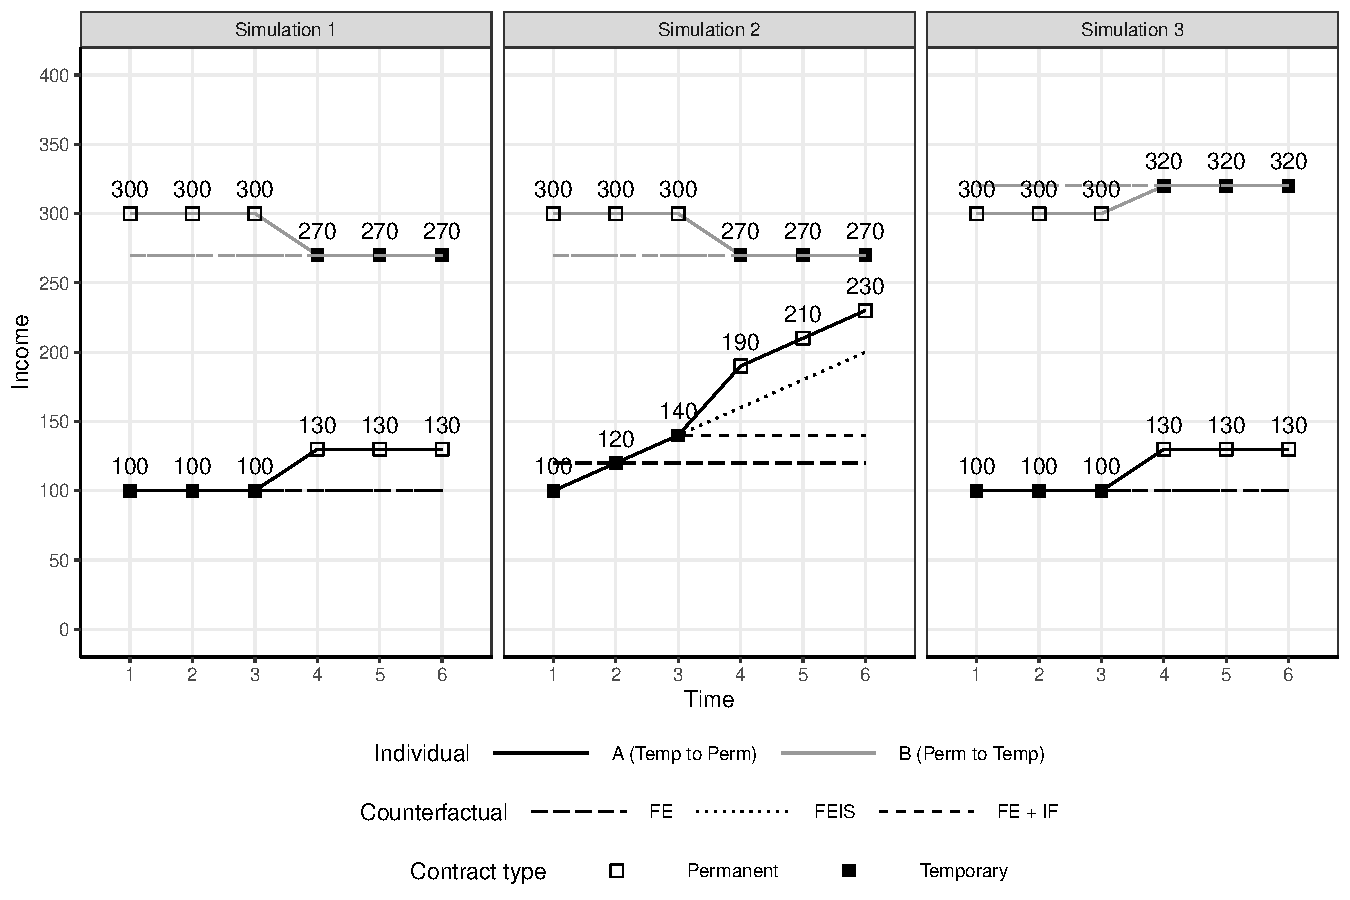
\includegraphics{../support_files/simulation/graphs/graph_compare_models_simulation_paper.pdf}}
    \label{graph_simulation}
\end{sidewaysfigure}

\begin{sidewaysfigure}[h!]
    \caption{Effect of event on wages at point in time}
    \resizebox{\textwidth}{!}{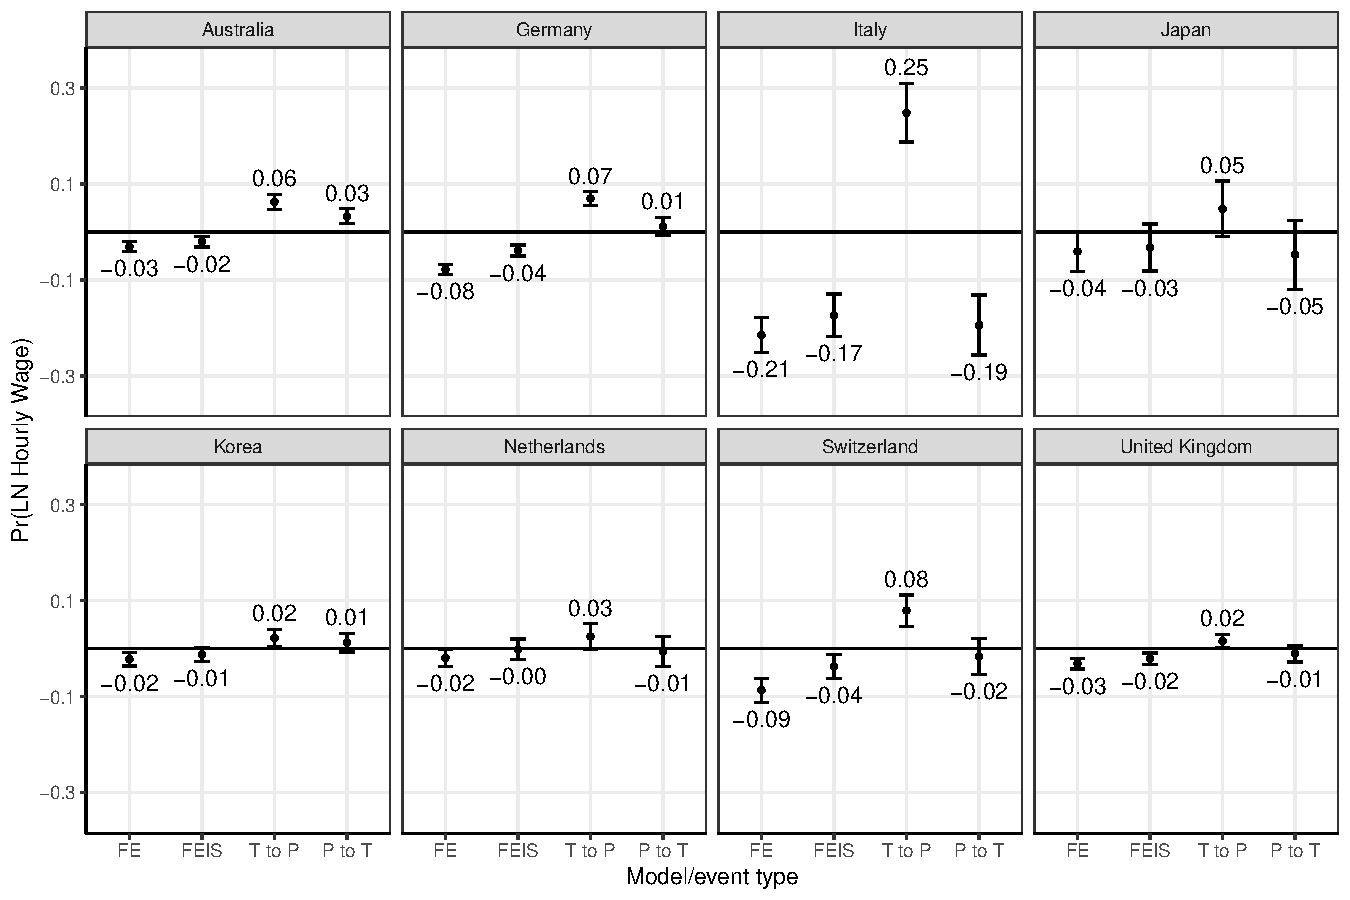
\includegraphics{../graphs/graph_multiple_events_contyp_paper.pdf}}
    \label{graph_contyp}
\end{sidewaysfigure}

\begin{sidewaysfigure}
    \caption{Effect of event on wages over time}
    \resizebox{\textwidth}{!}{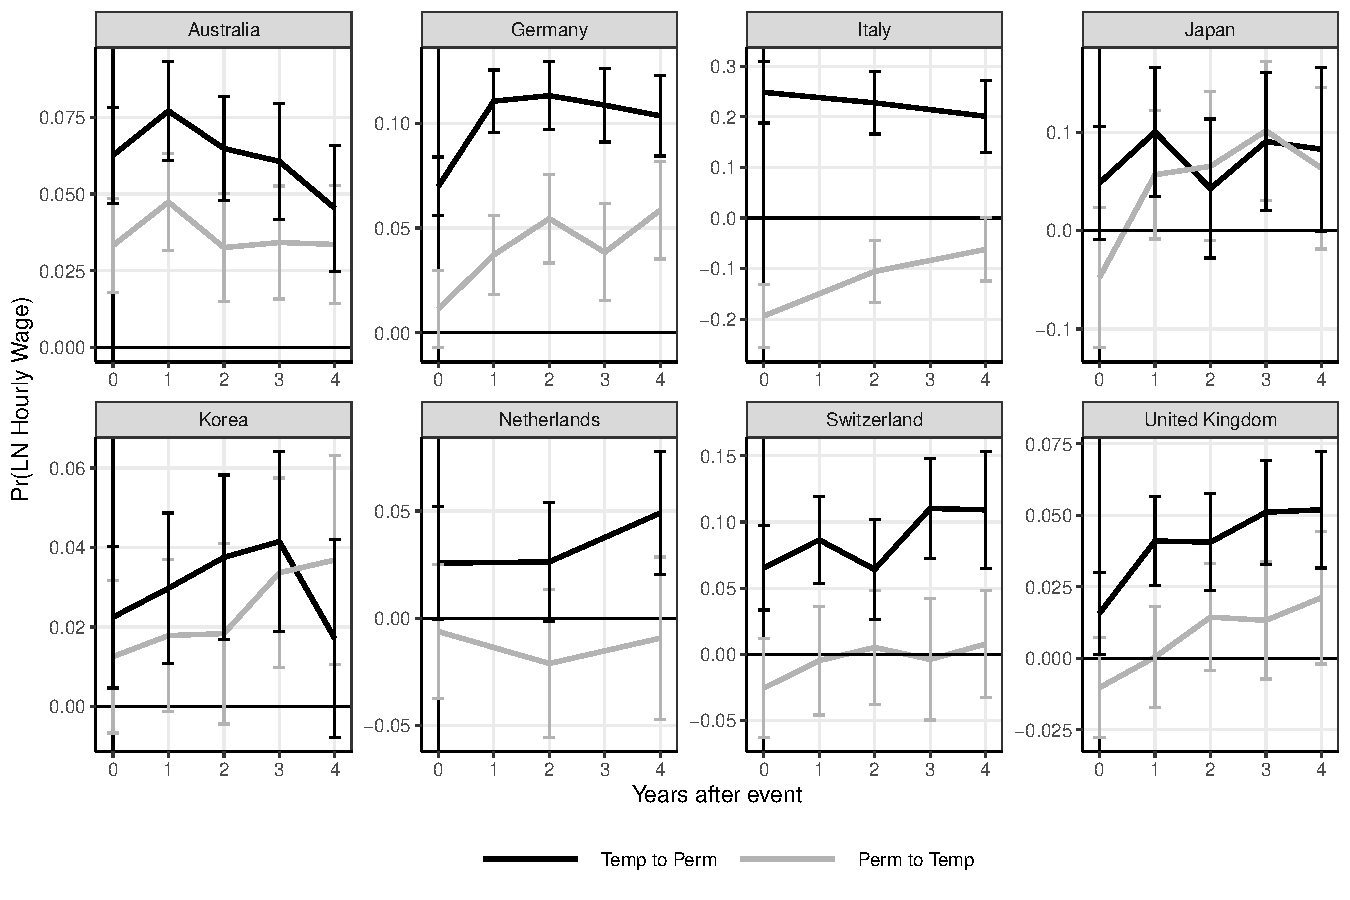
\includegraphics{../graphs/graph_multiple_events_contyp_post_paper.pdf}}
    \label{graph_contyp_post}
\end{sidewaysfigure}

\begin{sidewaysfigure}
    \caption{Effect of event on wages at point in time}
    \resizebox{\textwidth}{!}{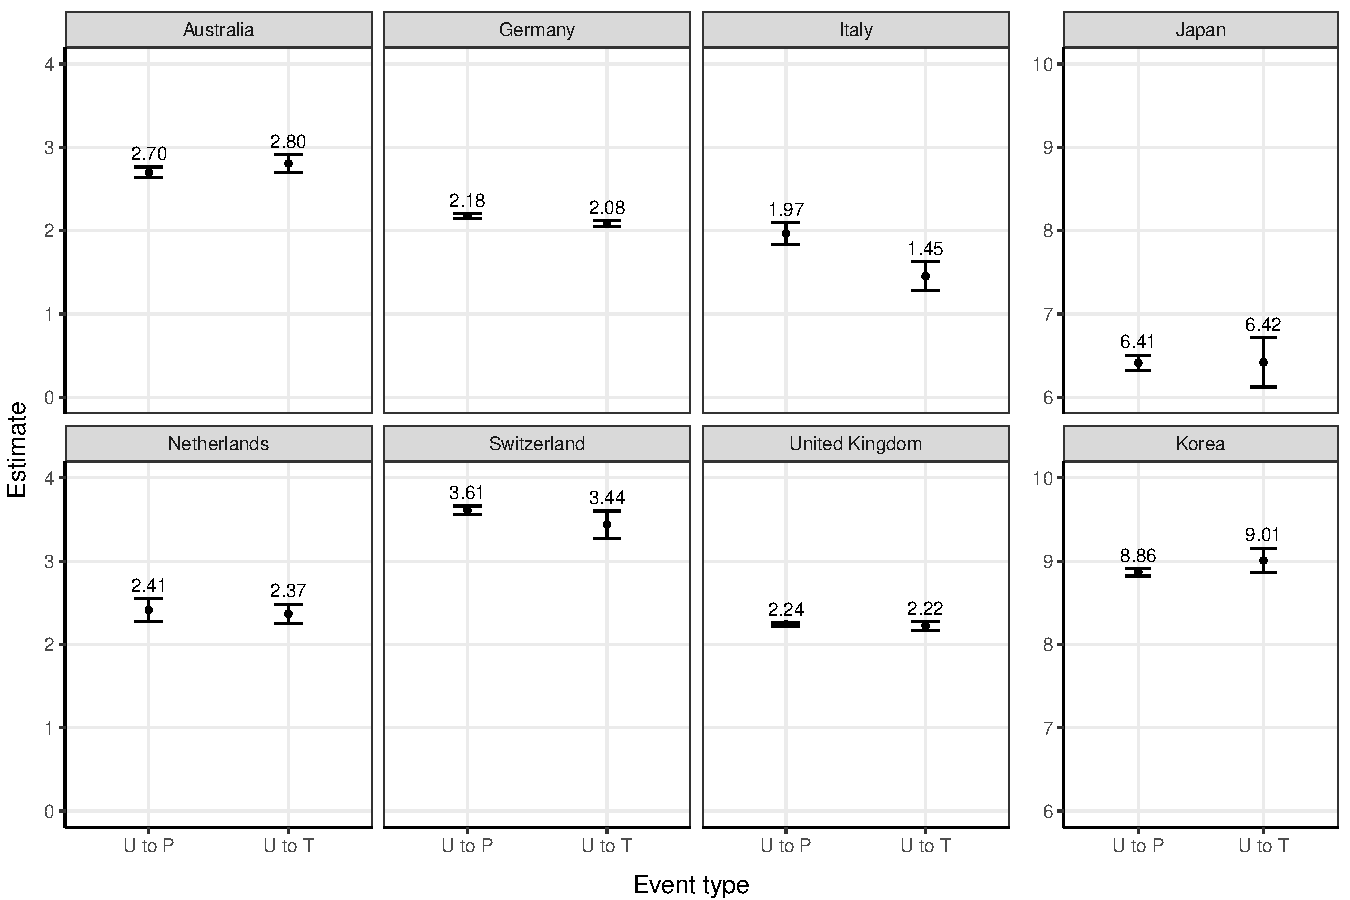
\includegraphics{../graphs/graph_multiple_events_unmp_better_paper.pdf}}
    \label{graph_unmp}
\end{sidewaysfigure}

\begin{sidewaysfigure}
    \caption{Graphical effect of event on wages over time}
    \resizebox{\textwidth}{!}{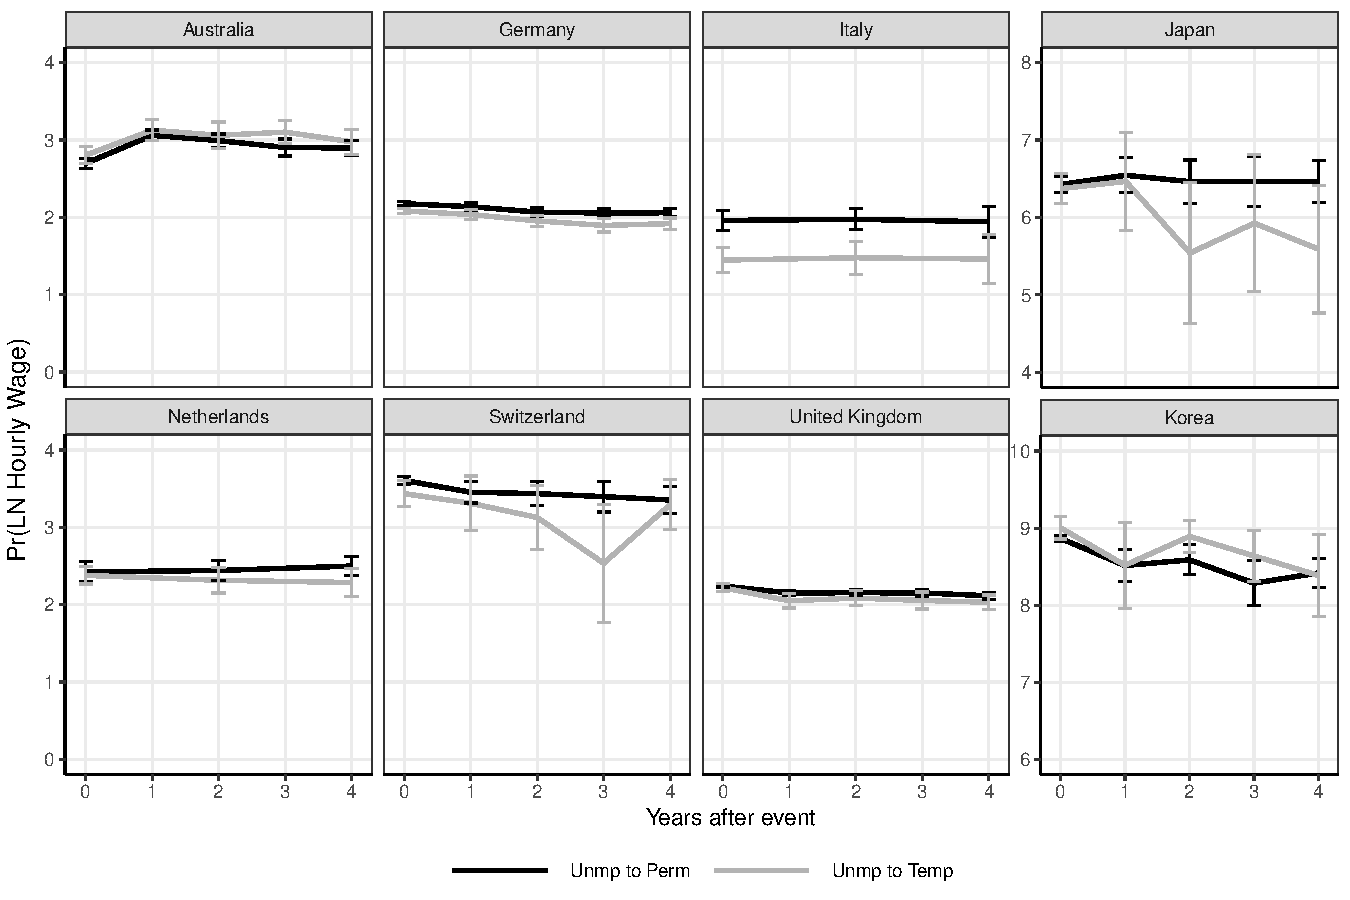
\includegraphics{../graphs/graph_multiple_events_unmp_post_better_paper.pdf}}
    \label{graph_unmp_post}
\end{sidewaysfigure}


%%%%%%%%%%%%%%%%%%%%%%%%%%%%%%%%%%%%%%%%%%
%%%%%%%%%%%%%%%%%%%%%%%%%%%%%%%%%%%%%%%%%%
%%%%%%%%%%%%%%%%%%%%%%%%%%%%%%%%%%%%%%%%%%
%%%%%%%%%%%%%%%%%%%%%%%%%%%%%%%%%%%%%%%%%%

%%%%%%%%%%%%%%%%%%%%%%%%%%
%APPENDIX
%%%%%%%%%%%%%%%%%%%%%%%%%%

\clearpage
\appendix
\setcounter{table}{0}
\setcounter{figure}{0}
\renewcommand*\thetable{\Alph{section}.\arabic{table}}
\renewcommand*\thefigure{\Alph{section}.\arabic{figure}}
\renewcommand{\theHfigure}{\Alph{section}.\arabic{table}}
\renewcommand{\theHtable}{\Alph{section}.\arabic{figure}}

\section{Appendix: Results sensitivity}\label{sec:sensitivity}

\begin{sidewaysfigure}[!h]
    \caption{Australia: All temporary (incl. casual) vs. FTC only (as in the paper)}
    \resizebox{\textwidth}{!}{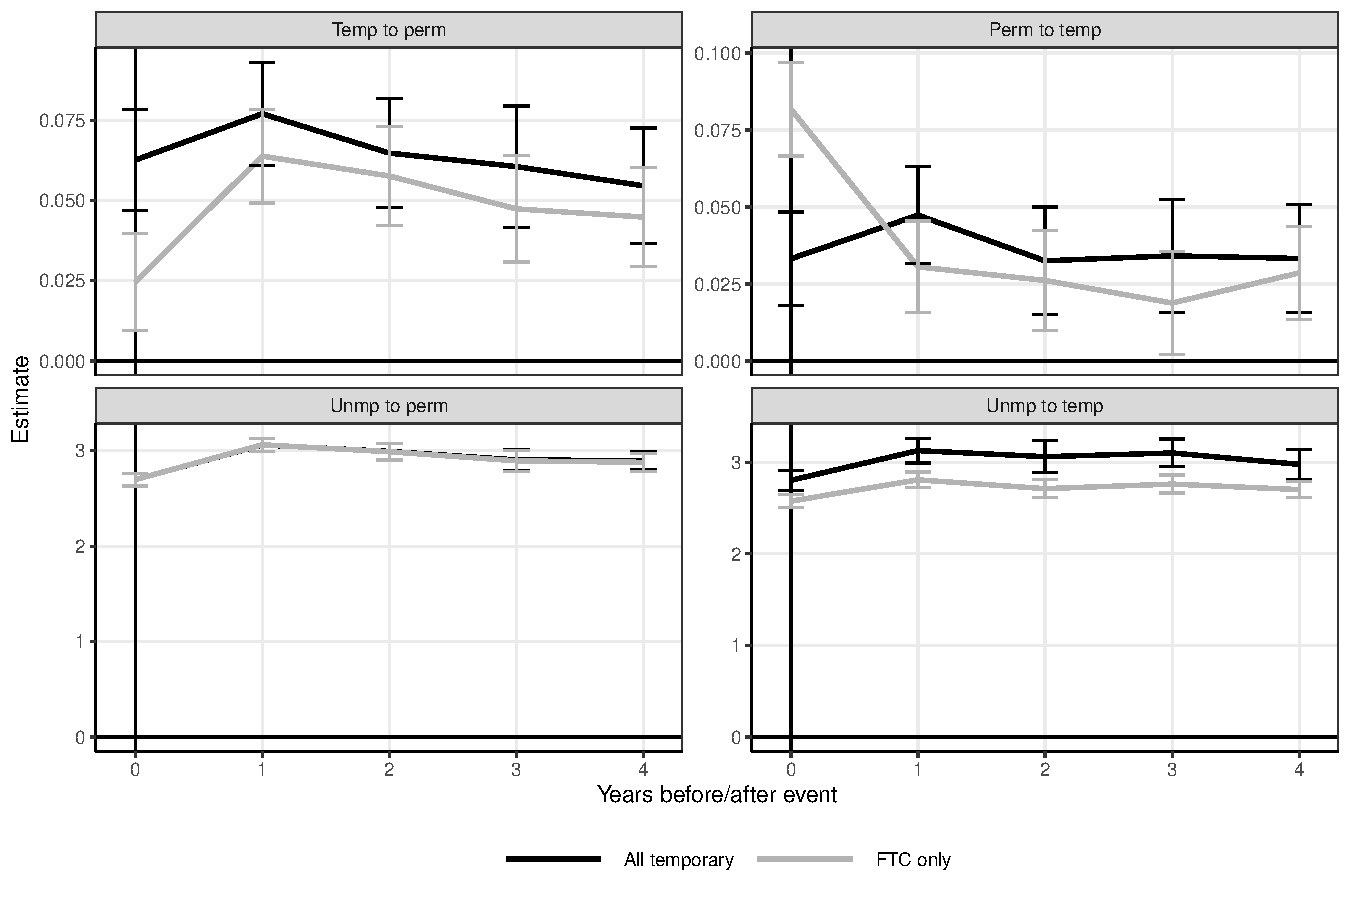
\includegraphics{../graphs/graph_sensitivity_AU_paper.pdf}}
    \label{graph_sensitivity_AU}
\end{sidewaysfigure}

\begin{sidewaysfigure}
    \caption{United Kingdom: All temporary (as in the paper) vs. FTC only}
    \resizebox{\textwidth}{!}{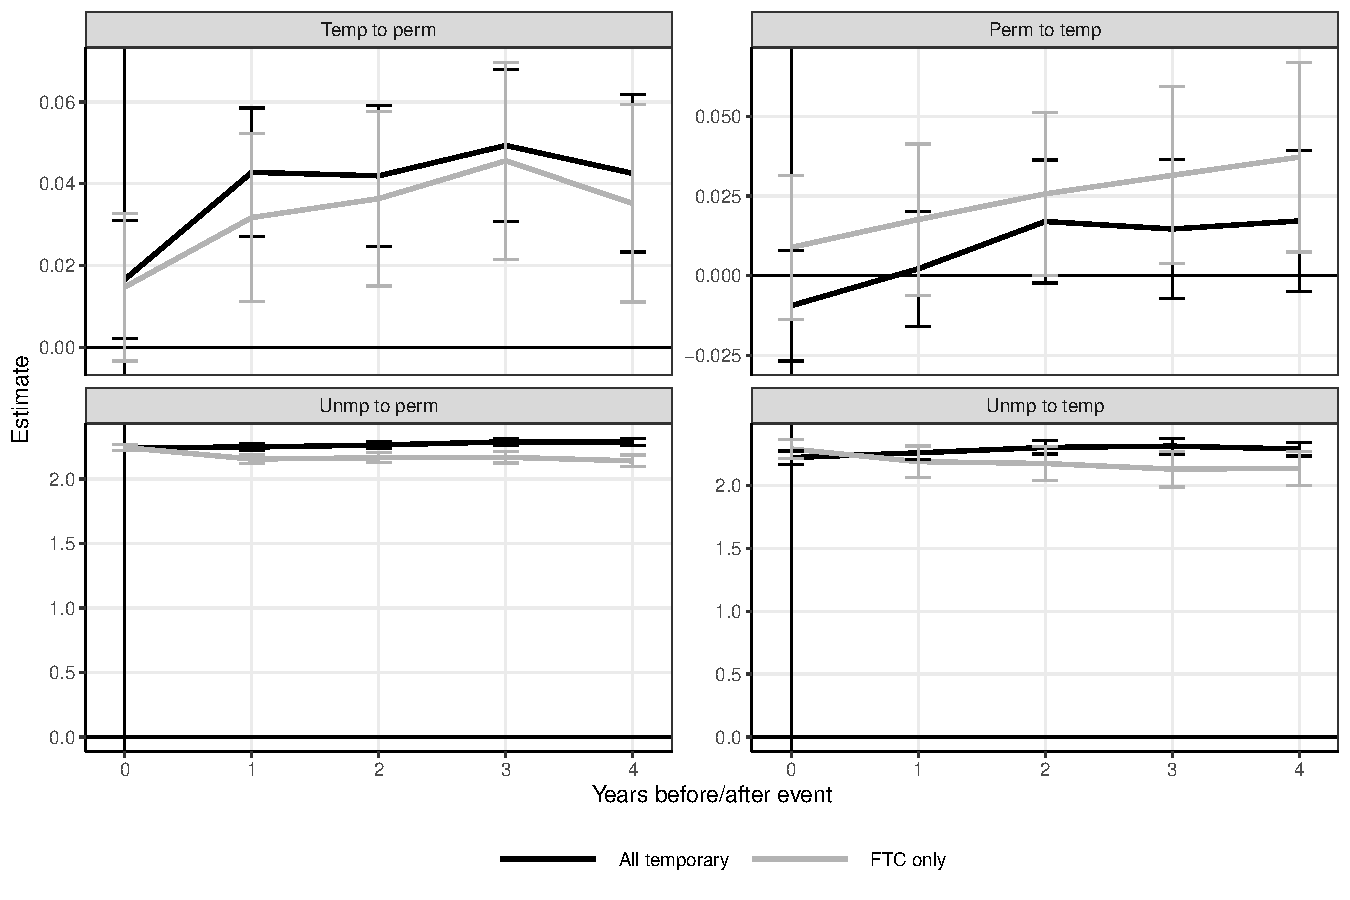
\includegraphics{../graphs/graph_sensitivity_UK_paper.pdf}}
    \label{graph_sensitivity_UK}
\end{sidewaysfigure}

\begin{sidewaysfigure}
    \caption{Netherlands: LSP (as in the paper) vs. LISS}
    \resizebox{\textwidth}{!}{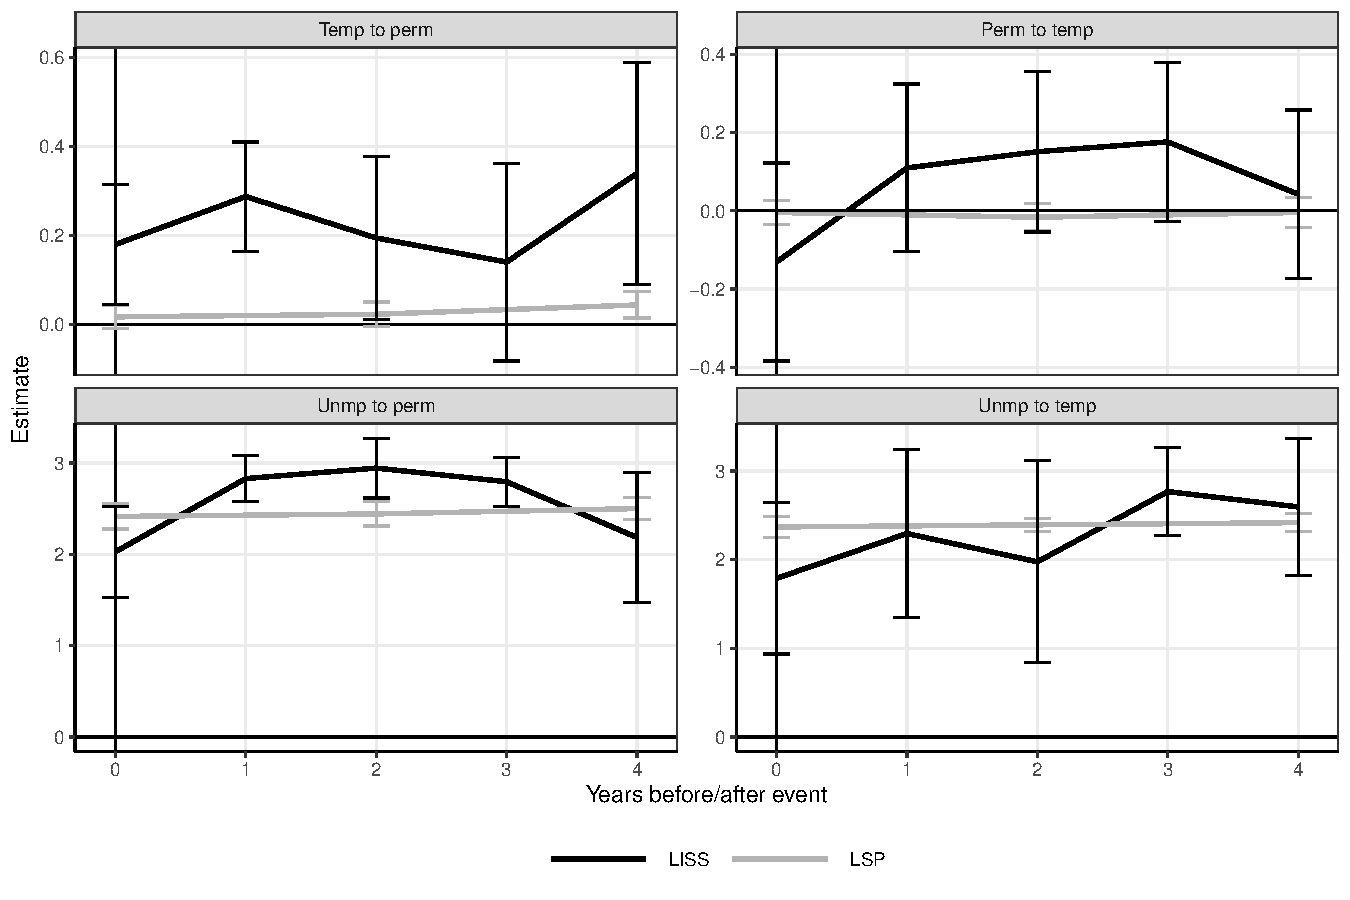
\includegraphics{../graphs/graph_sensitivity_NE_paper.pdf}}
    \label{graph_sensitivity_NE}
\end{sidewaysfigure}

\begin{sidewaysfigure}
    \caption{Methods: FE + IF (as in the paper) vs. FEIS + IF}
    \resizebox{\textwidth}{!}{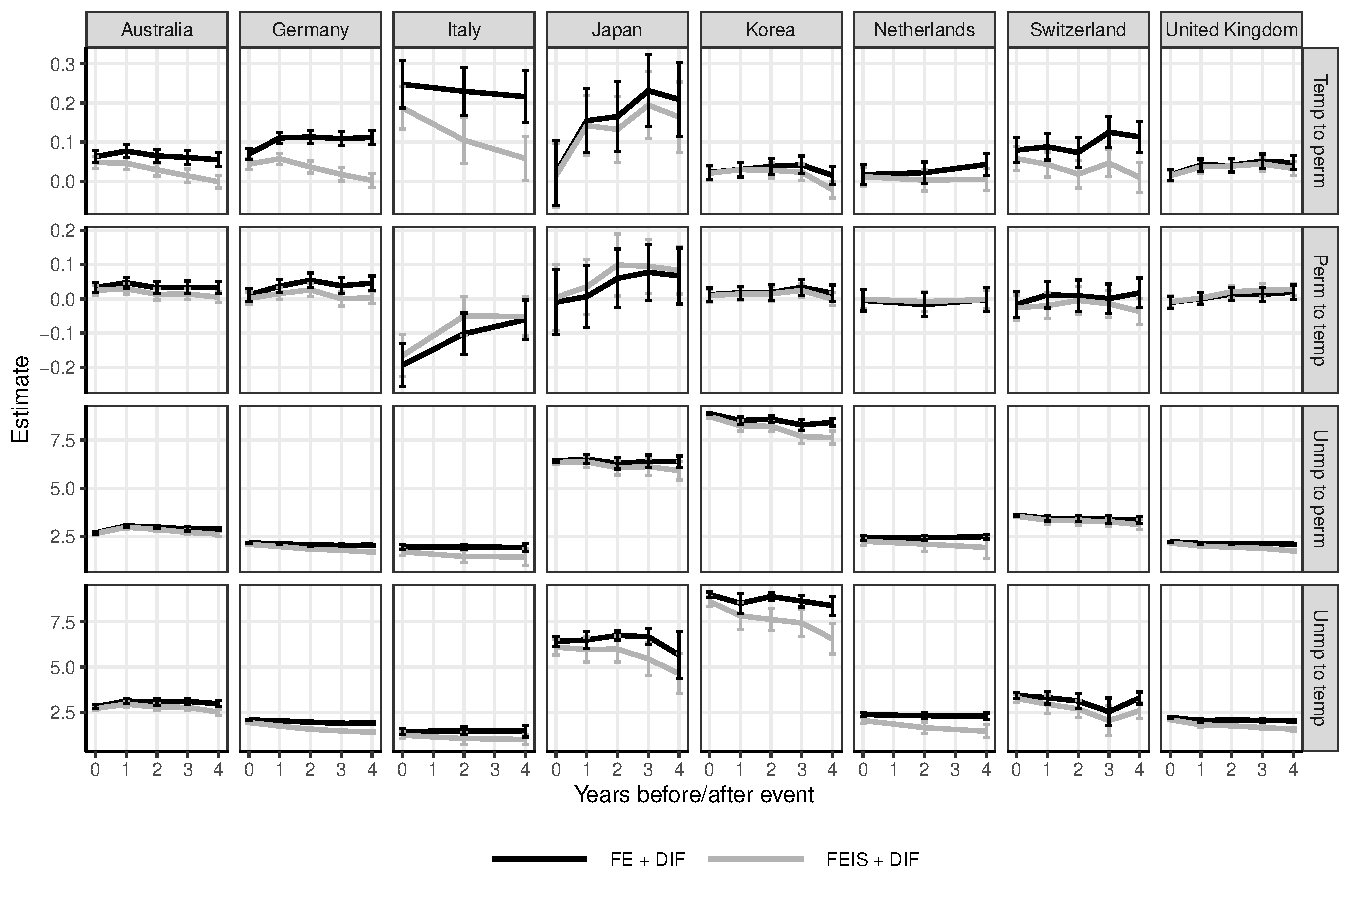
\includegraphics{../graphs/graph_compare_model_feis_paper.pdf}}
    \label{graph_compare_model_feis}
\end{sidewaysfigure}

%%%%%%%%%%%%%%%%%%%%%%%%%%%%%%%%%%%%%%%%%%
%%%%%%%%%%%%%%%%%%%%%%%%%%%%%%%%%%%%%%%%%%
%%%%%%%%%%%%%%%%%%%%%%%%%%%%%%%%%%%%%%%%%%
%%%%%%%%%%%%%%%%%%%%%%%%%%%%%%%%%%%%%%%%%%
\clearpage
\setcounter{table}{0}
\setcounter{figure}{0}
\renewcommand*\thetable{\Alph{section}.\arabic{table}}
\renewcommand*\thefigure{\Alph{section}.\arabic{figure}}
\renewcommand{\theHfigure}{\Alph{section}.\arabic{table}}
\renewcommand{\theHtable}{\Alph{section}.\arabic{figure}}

\section{Appendix: Results heterogeneity}\label{sec:heterogeneity}

\begin{sidewaysfigure}[!h]
    \caption{Figures \ref{graph_contyp_post} and \ref{graph_unmp_post}, by age category}
    \resizebox{\textwidth}{!}{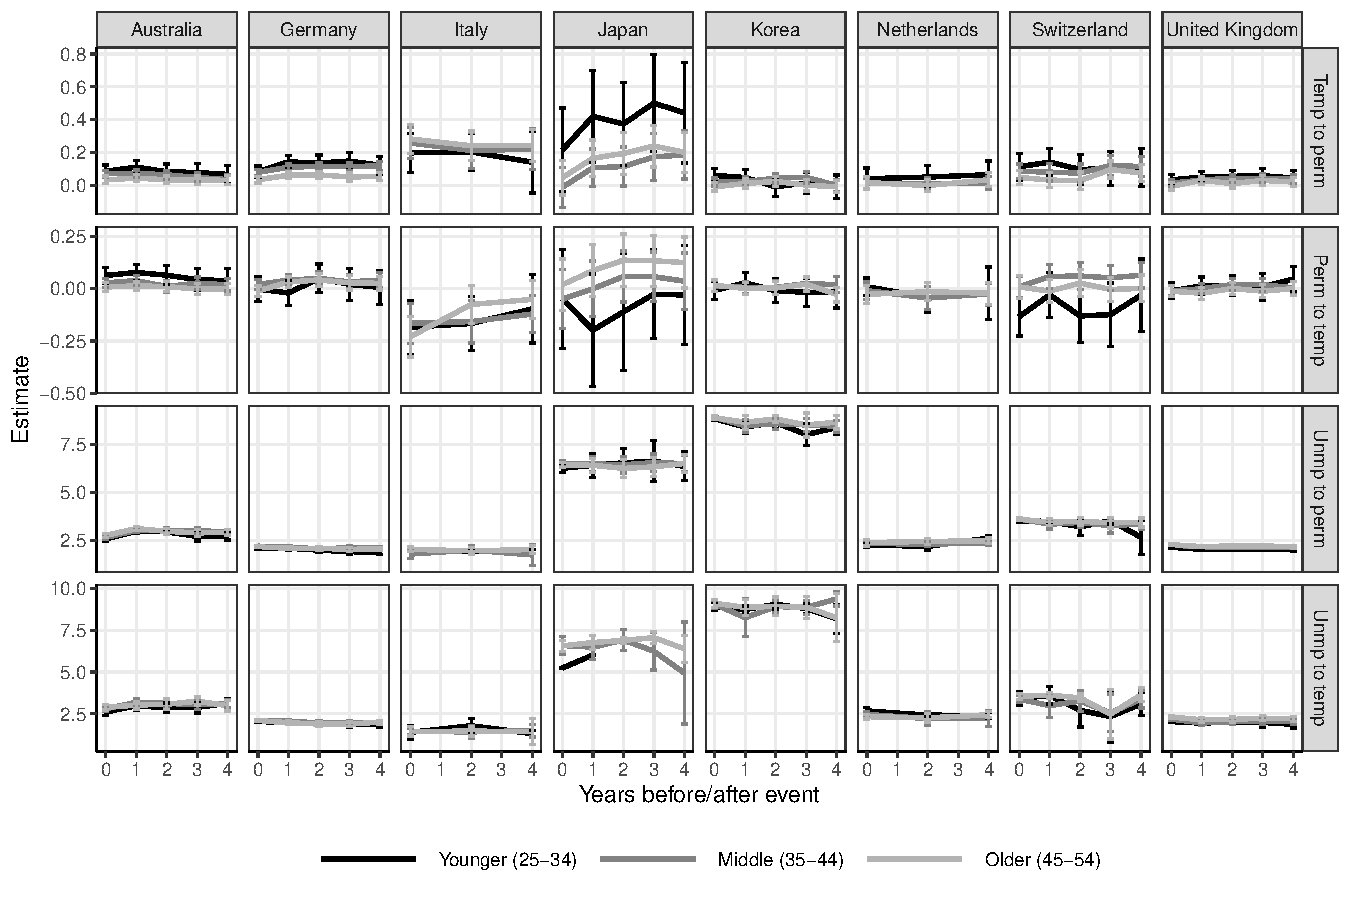
\includegraphics{../graphs/graph_post_event_age_cat.pdf}}
    \label{graph_post_event_age_cat}
\end{sidewaysfigure}

\begin{sidewaysfigure}[!h]
    \caption{Figures \ref{graph_contyp_post} and \ref{graph_unmp_post}, by education category}
    \resizebox{\textwidth}{!}{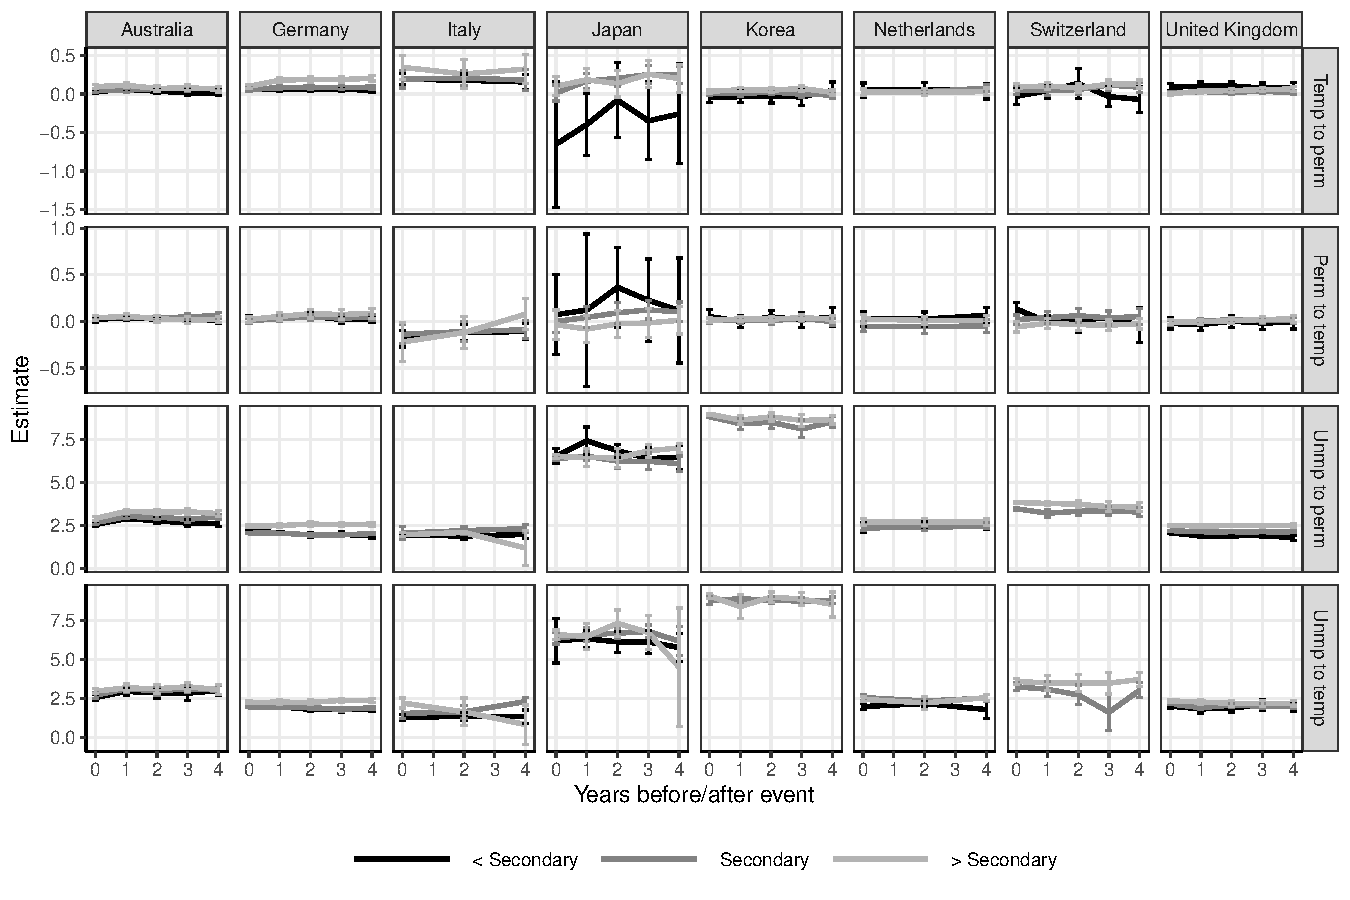
\includegraphics{../graphs/graph_post_event_edu_cat.pdf}}
    \label{graph_post_event_edu_cat}
\end{sidewaysfigure}

\begin{sidewaysfigure}[!h]
    \caption{Figures \ref{graph_contyp_post} and \ref{graph_unmp_post}, by gender}
    \resizebox{\textwidth}{!}{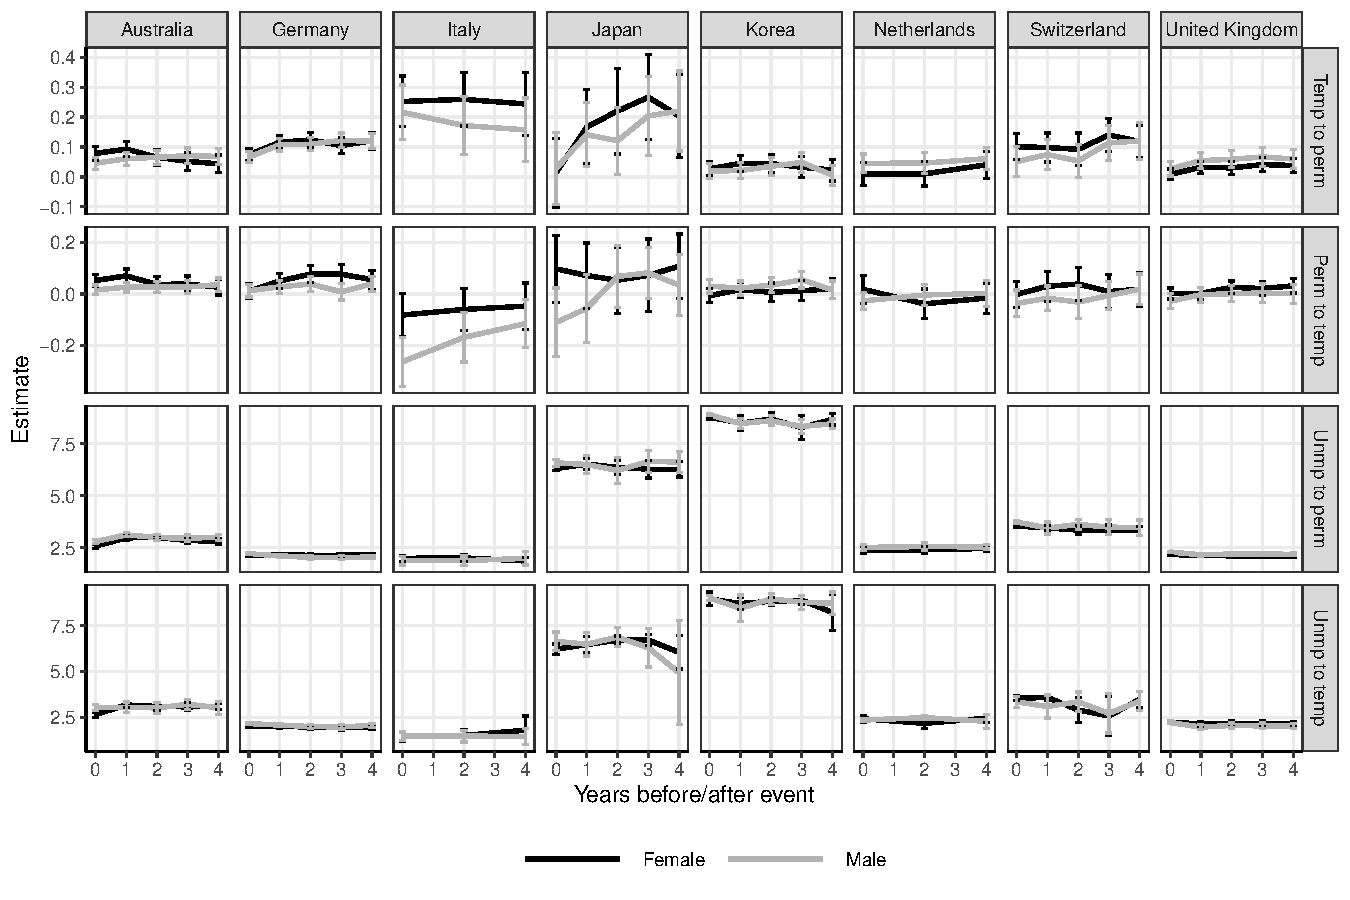
\includegraphics{../graphs/graph_post_event_gender.pdf}}
    \label{graph_post_event_gender}
\end{sidewaysfigure}

%%%%%%%%%%%%%%%%%%%%%%%%%%%%%%%%%%%%%%%%%%
%%%%%%%%%%%%%%%%%%%%%%%%%%%%%%%%%%%%%%%%%%
%%%%%%%%%%%%%%%%%%%%%%%%%%%%%%%%%%%%%%%%%%
%%%%%%%%%%%%%%%%%%%%%%%%%%%%%%%%%%%%%%%%%%
\clearpage
\section{Appendix: Multiple events}\label{sec:multiple}
\setcounter{figure}{0}    
\setcounter{table}{0}    
\renewcommand*\thetable{\Alph{section}.\arabic{table}}
\renewcommand*\thefigure{\Alph{section}.\arabic{figure}}
\renewcommand{\theHfigure}{\Alph{section}.\arabic{table}}
\renewcommand{\theHtable}{\Alph{section}.\arabic{figure}}

As shown in figure \ref{graph_compare_transformed}, let us imagine employment status for one individual in 6 periods of time looks like this (wages): T (50) $\rightarrow$ P (90) $\rightarrow$T (110) $\rightarrow$ P (130) $\rightarrow$ T (140) $\rightarrow$ T (150).  In this case, we may observe four distinct events T $\rightarrow$ P ($\times 2$), and P $\rightarrow$ T ($\times 2$).  In order to model each of the four distinct events, we must transform the data from person, year data into person, event, year data.

The steps are as follows.  First, for each individual, filter one row per individual, transition at the year which the transition occurs ($t_0$).  The result is four rows, one for each event.  Second, create two variables, one to identify each individual, transition ($transeq$) and a second variable for time ($eventtime$), which is 0.  Third, we create a new data frame by selecting only four variables: $pid$, $year$, $transseq$ and $eventtime$.  For each individual, transition ($transseq$), we append rows for $eventtime$ four years before and six years after the transition.  Finally, we merge the new data frame with the original data frame and create a new identifier for each individual, transition sequence ($pidseq$).   

The result is a new data frame with 24 rows: six observations per transition.  The transformed data do not alter the findings obtained by applying FE and FEIS models to untransformed data, as shown in table \ref{table_compare_transformed}.  

\begin{table}[!h]
    \caption{Simulation: Single individual with multiple events}
    \centering
    \resizebox{\textwidth}{!}{
\begin{tabular}{l c c c c c c c}
\toprule
 & \multicolumn{2}{c}{FE} & \multicolumn{2}{c}{FEIS} & \multicolumn{3}{c}{FE + IF} \\
\cmidrule(lr){2-3} \cmidrule(lr){4-5} \cmidrule(lr){6-8}
 & Original & Transformed & Original & Transformed & First & First & Multiple \\
\midrule
Temp                     & $2.50$ & $2.50^{***}$ & $-12.39$ & $-12.39^{***}$ &         &         &           \\
                         & $()$   & $(0.00)$     & $()$     & $(0.00)$       &         &         &           \\
Event: T $\rightarrow$ P &        &              &          &                & $40.00$ &         & $30.00$   \\
                         &        &              &          &                & $$      &         & $(13.05)$ \\
Event: P $\rightarrow$ T &        &              &          &                &         & $20.00$ & $15.00$   \\
                         &        &              &          &                &         & $()$    & $(6.53)$  \\
\midrule
Num. obs.                & $6$    & $24$         & $6$      & $24$           & $6$     & $6$     & $24$      \\
\bottomrule
\multicolumn{8}{l}{\scriptsize{$^{***}p<0.001$; $^{**}p<0.01$; $^{*}p<0.05$. Note: In FE + IF, pre and post event coefficients are not shown.}}
\end{tabular}
}
    \label{table_compare_transformed}
\end{table}

\begin{sidewaysfigure}[!h]
    \caption{Simulation: Single individual with multiple events}
    \resizebox{\textwidth}{!}{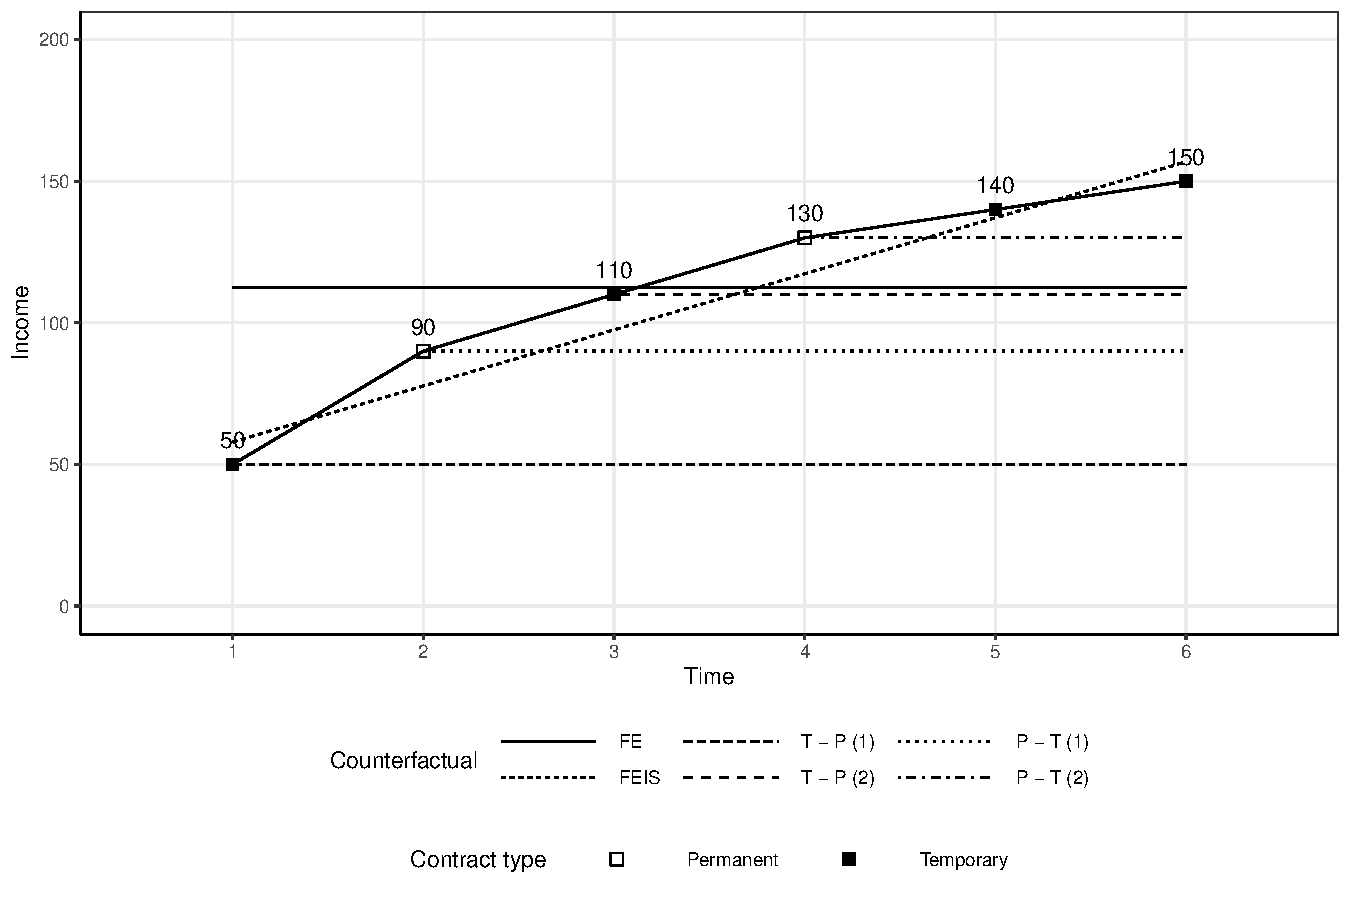
\includegraphics{../support_files/simulation/graphs/graph_compare_transformed_data_paper.pdf}}
    \label{graph_compare_transformed}
\end{sidewaysfigure}

\begin{sidewaysfigure}[!h]
    \caption{Compare single vs. multiple events}
    \resizebox{\textwidth}{!}{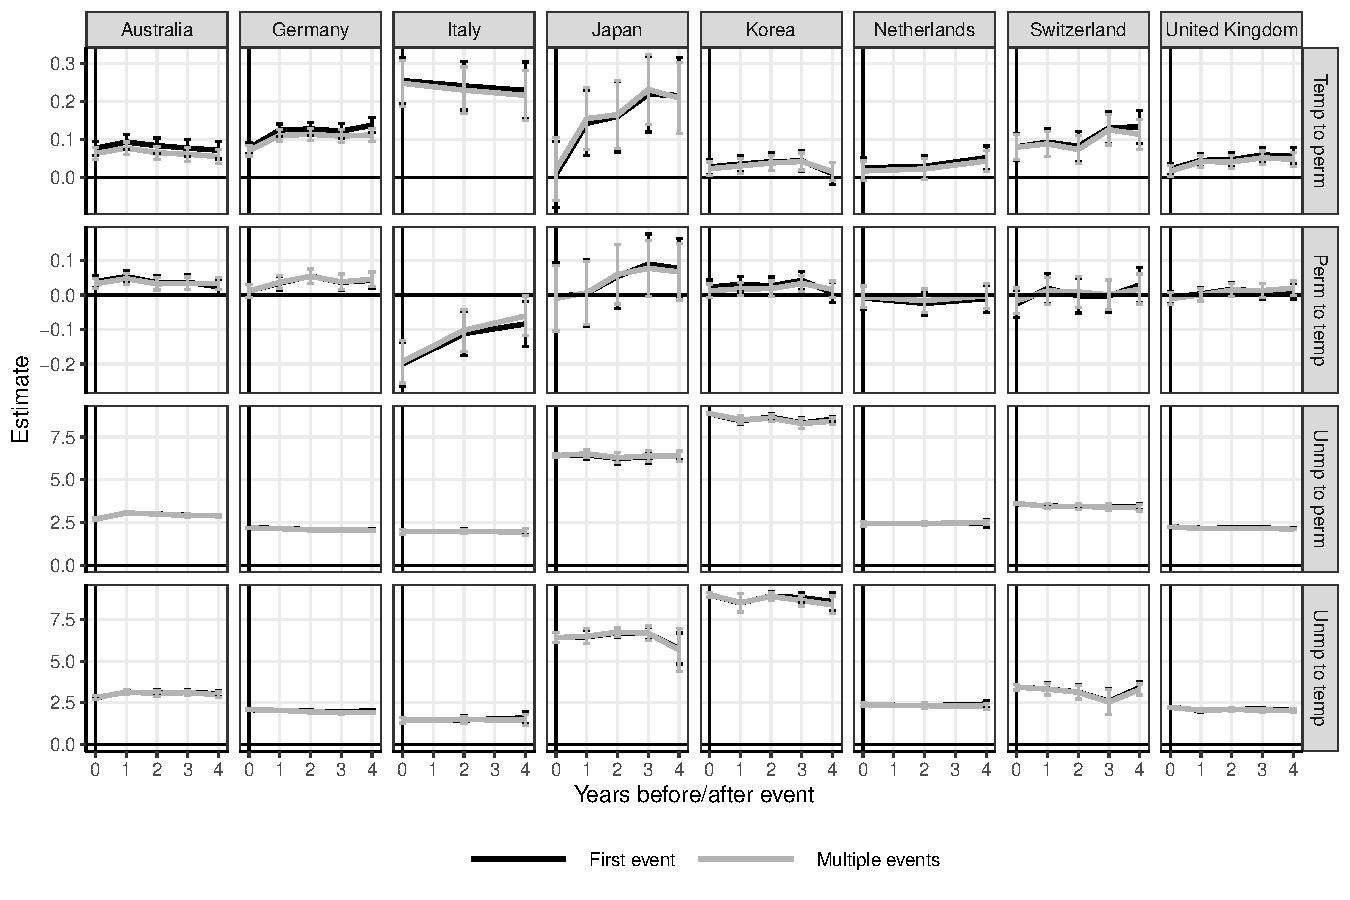
\includegraphics{../graphs/graph_sensitivity_single_multiple_events_paper.pdf}}
    \label{graph_sensitivity_single_multiple_events}
\end{sidewaysfigure}

\begin{sidewaysfigure}[!h]
    \caption{How many individuals experience multiple events?}
    \resizebox{\textwidth}{!}{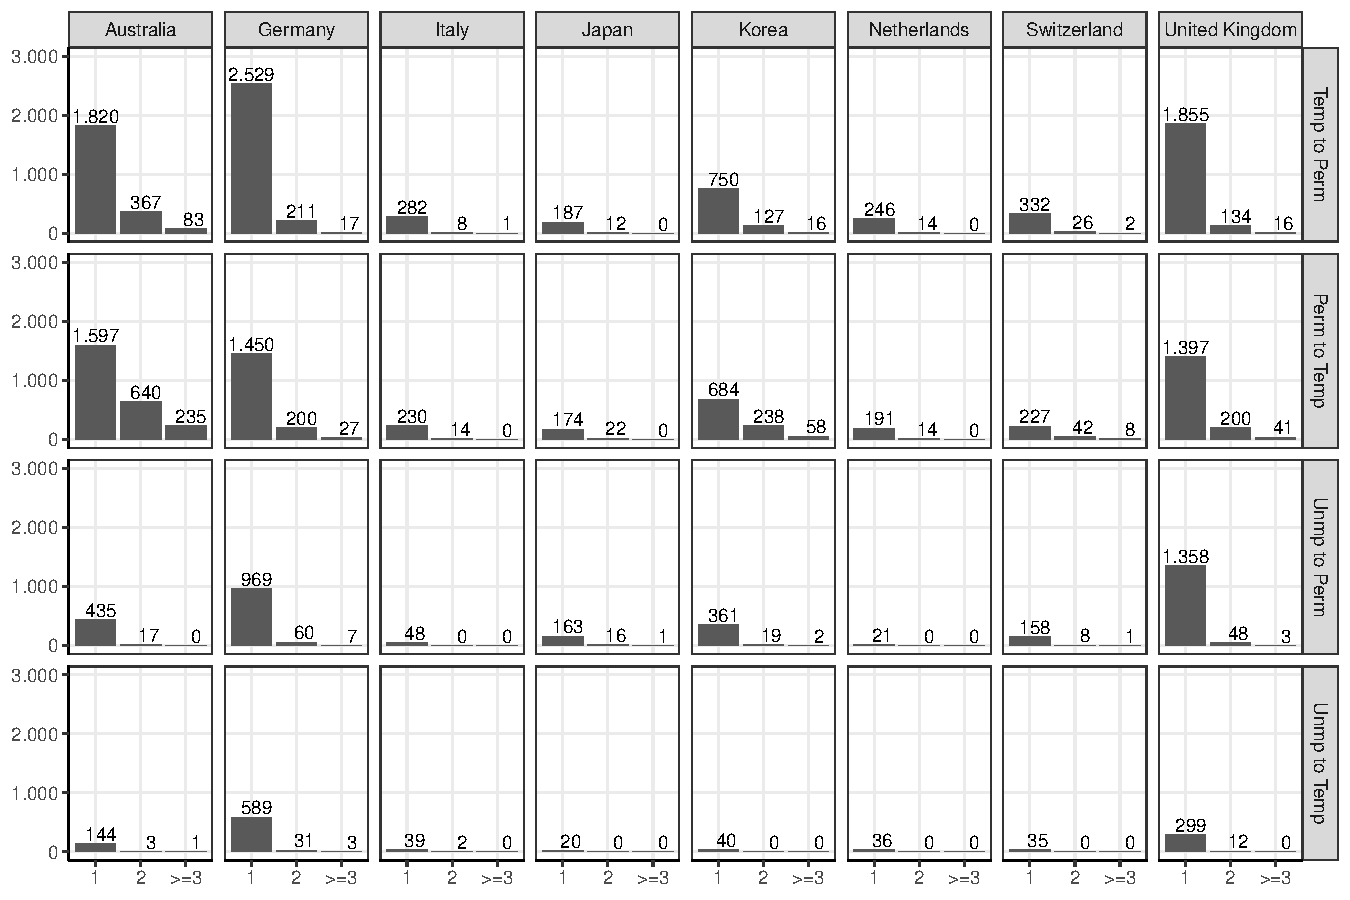
\includegraphics{../graphs/graph_country_events_multiple_presentation_num_paper.pdf}}
    \label{graph_country_events_multiple_presentation_num_paper}
\end{sidewaysfigure}

%%%%%%%%%%%%%%%%%%%%%%%%%%%%%%%%%%%%%%%%%%
%%%%%%%%%%%%%%%%%%%%%%%%%%%%%%%%%%%%%%%%%%
%%%%%%%%%%%%%%%%%%%%%%%%%%%%%%%%%%%%%%%%%%
%%%%%%%%%%%%%%%%%%%%%%%%%%%%%%%%%%%%%%%%%%
\clearpage
\section{Appendix: Sample selection}\label{sec:sample_selection}
\setcounter{figure}{0}    
\setcounter{table}{0}    
\renewcommand*\thetable{\Alph{section}.\arabic{table}}
\renewcommand*\thefigure{\Alph{section}.\arabic{figure}}
\renewcommand{\theHfigure}{\Alph{section}.\arabic{table}}
\renewcommand{\theHtable}{\Alph{section}.\arabic{figure}}

In this appendix, we provide more detail about the sample selection criteria.  Table \ref{table_sample_filter_steps} in the paper details the sample selection criteria, which reduces the sample size by over 50\% in a given country.  Table \ref{table_sample_filter_steps_country} splits table \ref{table_sample_filter_steps} for country.  Table \ref{table_sample_unmp_steps_contyp} specifies why the number of transitions from unemployment to temporary or permanent employment are so small.  The answer is that only about half of individuals who experience unemployment, exit unemployment, and only about a quarter of those who exit are observable as employed within 5 years after the transition (i.e. 3 periods of observation).  More generally, despite sample selection criteria, sample A and B provide similar estimates in a given country, year of average income (LN), unemployment rate, and temporary employment rate as the World Bank  or OECD.  Therefore, the sample are representative of the broader population in a given country.

\begin{sidewaystable}[!h]
    \caption{Sample filter steps from table \ref{table_sample_filter_steps}, by country}
    \centering
    \resizebox{\textwidth}{!}{\begin{tabular}{l>{\raggedright\arraybackslash}p{2.5in}llllllllllllllllll}
   \toprule 
 
\multicolumn{14}{l}{{\bf Panel A:} Sample selection criteria} \\ 

&  & 
\multicolumn{2}{l}{Total (all countries)} &
\multicolumn{2}{l}{Australia} &
\multicolumn{2}{l}{Germany} &
\multicolumn{2}{l}{Italy} &
\multicolumn{2}{l}{Japan} &
\multicolumn{2}{l}{Korea} &
\multicolumn{2}{l}{Netherlands} &
\multicolumn{2}{l}{Switzerland} &
\multicolumn{2}{l}{United Kingdom}
\\  
 
 
\multicolumn{1}{l}{Step} & 
\multicolumn{1}{l}{Description} 
& n & $\Delta$
& n & $\Delta$
& n & $\Delta$
& n & $\Delta$
& n & $\Delta$
& n & $\Delta$
& n & $\Delta$
& n & $\Delta$
& n & $\Delta$
\\ 
\cmidrule(lr){1-2}
\cmidrule(lr){3-4}
\cmidrule(lr){5-6}
\cmidrule(lr){7-8}
\cmidrule(lr){9-10}
\cmidrule(lr){11-12}
\cmidrule(lr){13-14}
\cmidrule(lr){15-16}
\cmidrule(lr){17-18}
\cmidrule(lr){19-20}
\\[-1.8ex]  
 
0 & Raw data & 415,771 &  & 31,951 &  & 91,693 &  & 100,847 &  & 10,499 &  & 24,491 &  & 14,458 &  & 34,469 &  & 107,363 &  \\ 
  1 & Panel years between 2000 and 2018 & 367,032 & -12\% & 31,951 & 0\% & 83,722 & -9\% & 68,012 & -33\% & 10,499 & 0\% & 23,515 & -4\% & 14,458 & 0\% & 34,469 & 0\% & 100,406 & -6\% \\ 
  2 & Prime age (25 - 54) & 210,900 & -43\% & 19,431 & -39\% & 52,198 & -38\% & 33,724 & -50\% & 6,315 & -40\% & 16,089 & -32\% & 9,693 & -33\% & 17,205 & -50\% & 56,245 & -44\% \\ 
  3 & Unemployed or employed with contract type, monthly hours (40 -- 320), and wages $>$ 0 & 157,370 & -25\% & 15,881 & -18\% & 38,538 & -26\% & 25,547 & -24\% & 4,787 & -24\% & 10,980 & -32\% & 7,461 & -23\% & 9,251 & -46\% & 44,925 & -20\% \\ 
  4 & Non missing education or gender & 155,535 & -1\% & 15,875 & 0\% & 37,635 & -2\% & 25,547 & 0\% & 4,767 & 0\% & 10,978 & 0\% & 7,449 & 0\% & 9,251 & 0\% & 44,033 & -2\% \\ 
  5 & Hourly wages within the top/bottom 0.005 percentile & 154,743 & -1\% & 15,817 & 0\% & 37,454 & 0\% & 25,336 & -1\% & 4,754 & 0\% & 10,943 & 0\% & 7,404 & -1\% & 9,168 & -1\% & 43,867 & 0\% \\ 
  6 & Data set A: At least 3 observations & 79,148 & -49\% & 10,598 & -33\% & 20,972 & -44\% & 3,678 & -85\% & 3,179 & -33\% & 7,311 & -33\% & 2,418 & -67\% & 5,303 & -42\% & 25,689 & -41\% \\ 
  7 & Data set B: + always employed & 73,189 & -8\% & 10,072 & -5\% & 18,302 & -13\% & 3,449 & -6\% & 3,079 & -3\% & 7,103 & -3\% & 2,320 & -4\% & 5,153 & -3\% & 23,711 & -8\% \\ 
   
\hline \\[-1.8ex]  
 
\multicolumn{14}{l}{{\bf Panel B:} Data sets by event type (if treated, must be employed after treatment)} \\ 

& 
& \# & \%
& \# & \%
& \# & \%
& \# & \%
& \# & \%
& \# & \%
& \# & \%
& \# & \%
& \# & \%
\\ 
\cmidrule(lr){1-2}
\cmidrule(lr){3-4}
\cmidrule(lr){5-6}
\cmidrule(lr){7-8}
\cmidrule(lr){9-10}
\cmidrule(lr){11-12}
\cmidrule(lr){13-14}
\cmidrule(lr){15-16}
\cmidrule(lr){17-18}
\cmidrule(lr){19-20}
\\[-1.8ex]  
 
A & Unmp $\rightarrow$ perm & 3,670 & 5\% & 452 & 4\% & 1,036 & 5\% & 48 & 1\% & 155 & 5\% & 382 & 5\% & 21 & 1\% & 167 & 3\% & 1,409 & 5\% \\ 
  A & Unmp $\rightarrow$ temp & 1,268 & 2\% & 148 & 1\% & 623 & 3\% & 41 & 1\% & 34 & 1\% & 40 & 1\% & 36 & 1\% & 35 & 1\% & 311 & 1\% \\ 
  B & Temp $\rightarrow$ perm & 9,063 & 12\% & 2,270 & 23\% & 2,757 & 15\% & 291 & 8\% & 227 & 7\% & 893 & 13\% & 260 & 11\% & 360 & 7\% & 2,005 & 8\% \\ 
  B & Perm $\rightarrow$ temp & 6,800 & 9\% & 1,992 & 20\% & 1,559 & 9\% & 237 & 7\% & 232 & 8\% & 822 & 12\% & 198 & 9\% & 250 & 5\% & 1,510 & 6\% \\ 
   \bottomrule \\[-1.8ex] \multicolumn{20}{p{12in}}{Note: n - is unique observations.  $\Delta$ - is difference in n from previous step.  \# - is unique n who experienced at least 1 event.  \% - is percent who experienced an event.} 
\end{tabular}
}
    \label{table_sample_filter_steps_country}
\end{sidewaystable}

\begin{sidewaystable}[!h]
    \caption{Why are the number of unemployment exits so small?}
    \centering
    \resizebox{\textwidth}{!}{\begin{tabular}{l>{\raggedright\arraybackslash}p{2in}llllllllllllllllll}
   \\[-1.8ex]\hline\hline \\ 
 [-1.8ex]
\multicolumn{20}{l}{{\bf Panel A:} Sample selection criteria} \\ 

&  & 
\multicolumn{2}{l}{Total (all countries)} &
\multicolumn{2}{l}{Australia} &
\multicolumn{2}{l}{Germany} &
\multicolumn{2}{l}{Italy} &
\multicolumn{2}{l}{Japan} &
\multicolumn{2}{l}{Korea} &
\multicolumn{2}{l}{Netherlands} &
\multicolumn{2}{l}{Switzerland} &
\multicolumn{2}{l}{United Kingdom}
\\  
 
 
\multicolumn{1}{l}{Step} & 
\multicolumn{1}{l}{Description} 
& n & $\Delta$
& n & $\Delta$
& n & $\Delta$
& n & $\Delta$
& n & $\Delta$
& n & $\Delta$
& n & $\Delta$
& n & $\Delta$
& n & $\Delta$
\\ 
\cmidrule(lr){1-2}
\cmidrule(lr){3-4}
\cmidrule(lr){5-6}
\cmidrule(lr){7-8}
\cmidrule(lr){9-10}
\cmidrule(lr){11-12}
\cmidrule(lr){13-14}
\cmidrule(lr){15-16}
\cmidrule(lr){17-18}
\cmidrule(lr){19-20}
\\[-1.8ex]  
 
1 & Total unemployment events (From data set A) & 14,450 &  & 1,917 &  & 5,562 &  & 335 &  & 364 &  & 980 &  & 184 &  & 531 &  & 4,577 &  \\ 
  2 & Must exit unemployment & 6,463 & -55\% & 1,060 & -45\% & 2,079 & -63\% & 145 & -57\% & 212 & -42\% & 478 & -51\% & 90 & -51\% & 256 & -52\% & 2,143 & -53\% \\ 
  3 & Employed at least 1 period after exit (within 5 years) & 4,847 & -25\% & 592 & -44\% & 1,608 & -23\% & 86 & -41\% & 184 & -13\% & 419 & -12\% & 56 & -38\% & 199 & -22\% & 1,703 & -21\% \\ 
   
\hline \\[-1.8ex]  
 
\multicolumn{20}{l}{{\bf Panel B:} Frequency, by event type} \\ 

& 
&  \# & \%
&  \# & \%
&  \# & \%
&  \# & \%
&  \# & \%
&  \# & \%
&  \# & \%
&  \# & \%
&  \# & \%
\\ 
\cmidrule(lr){1-2}
\cmidrule(lr){3-4}
\cmidrule(lr){5-6}
\cmidrule(lr){7-8}
\cmidrule(lr){9-10}
\cmidrule(lr){11-12}
\cmidrule(lr){13-14}
\cmidrule(lr){15-16}
\cmidrule(lr){17-18}
\cmidrule(lr){19-20}
\\[-1.8ex]  
 
 & Unmp $\rightarrow$ temp & 1,268 & 26\% & 148 & 25\% & 623 & 39\% & 41 & 48\% & 34 & 18\% & 40 & 10\% & 36 & 64\% & 35 & 18\% & 311 & 18\% \\ 
   & Unmp $\rightarrow$ perm & 3,670 & 76\% & 452 & 76\% & 1,036 & 64\% & 48 & 56\% & 155 & 84\% & 382 & 91\% & 21 & 38\% & 167 & 84\% & 1,409 & 83\% \\ 
   & U $\rightarrow$ P \& U $\rightarrow$ T & 91 &  & 8 &  & 51 &  & 3 &  & 5 &  & 3 &  & 1 &  & 3 &  & 17 &  \\ 
   \hline \\[-1.8ex] \multicolumn{20}{p{12in}}{Notes: n - is unique observations.  
               $\Delta$ - is difference in n from previous step.  
               \# - is number of transitions.  
               \% - is percent of total transitions from step 3. 
               \% is more than 100\% because some individuals experience both a transition from Unmp to Perm and Unmp to Temp.} 
\end{tabular}
}
    \label{table_sample_unmp_steps_contyp}
\end{sidewaystable}



\begin{sidewaysfigure}[!h]
    \caption{Compare annual average income (LN) from sample to OECD}
    \resizebox{\textwidth}{!}{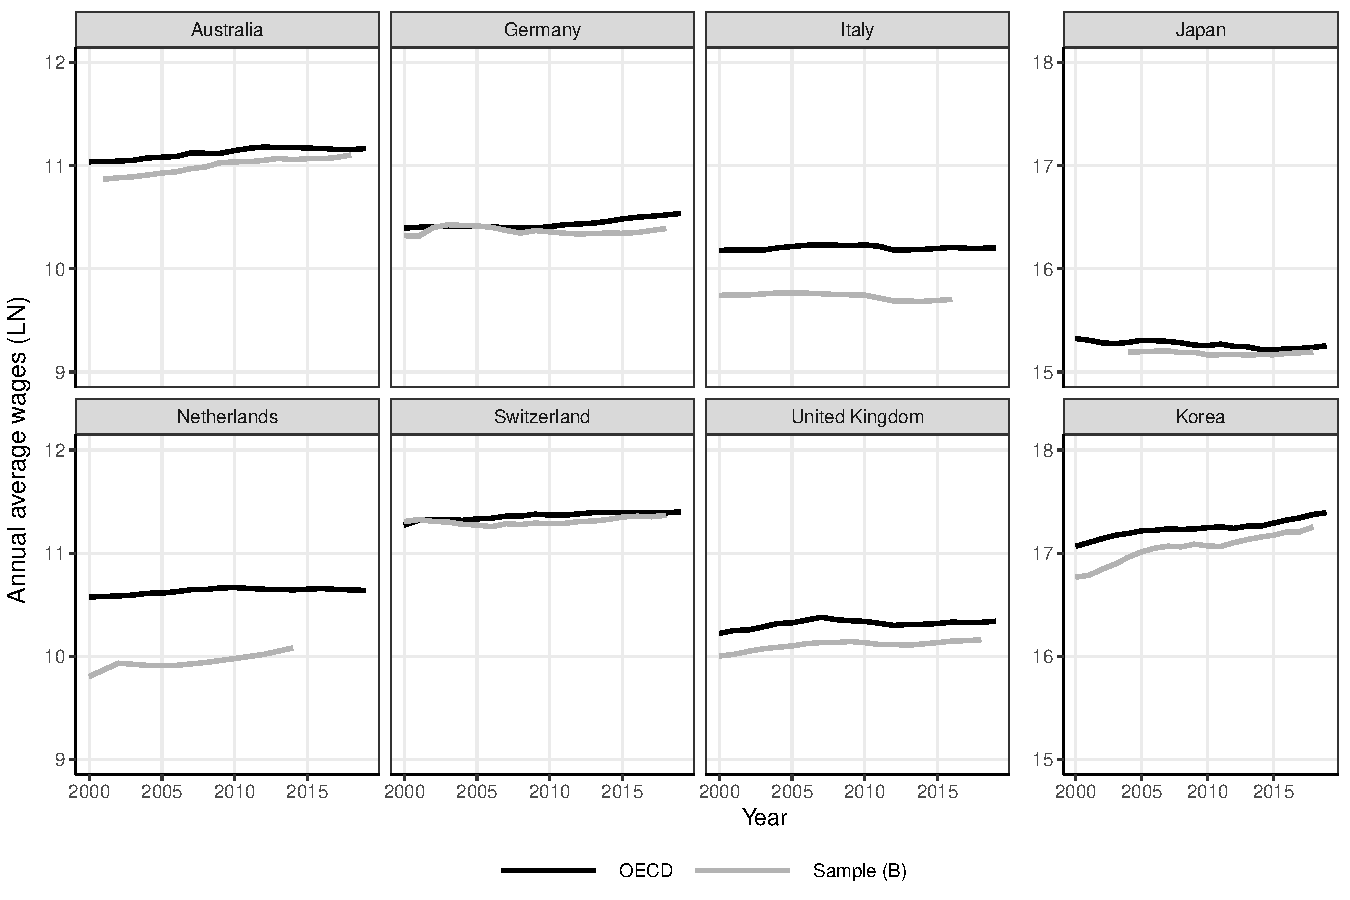
\includegraphics{../graphs/graph_descriptives_income_better_paper.pdf}}
    \label{graph_descriptives_income_better_paper.pdf}
\end{sidewaysfigure}

\begin{sidewaysfigure}[!h]
    \caption{Compare unemployment rate from sample to World Bank}
    \resizebox{\textwidth}{!}{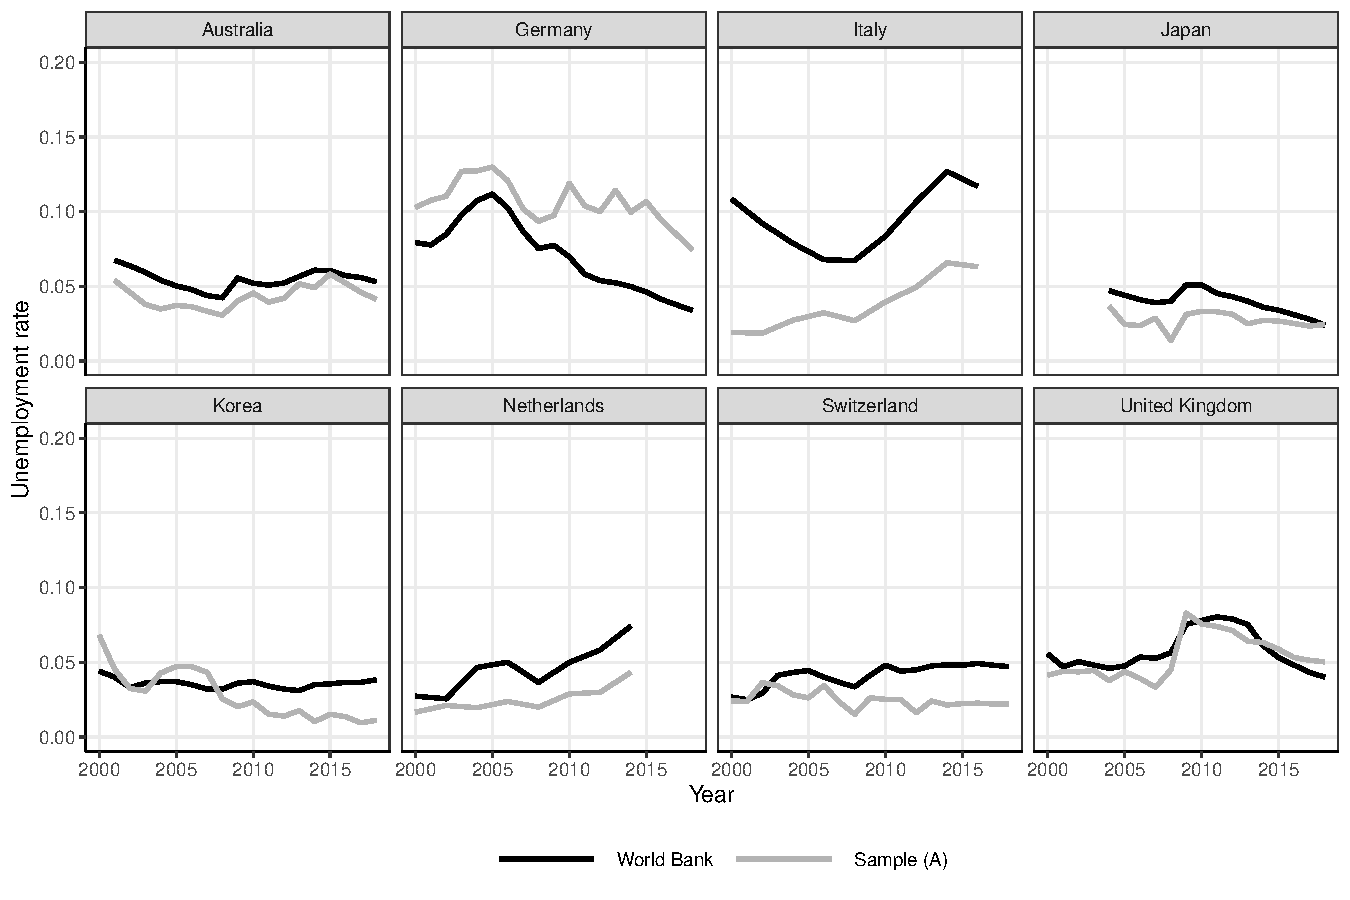
\includegraphics{../graphs/graph_descriptives_unmp_paper.pdf}}
    \label{graph_descriptives_unmp_paper}
\end{sidewaysfigure}

\begin{sidewaysfigure}[!h]
    \caption{Compare temporary employment rate from sample to OECD}
    \resizebox{\textwidth}{!}{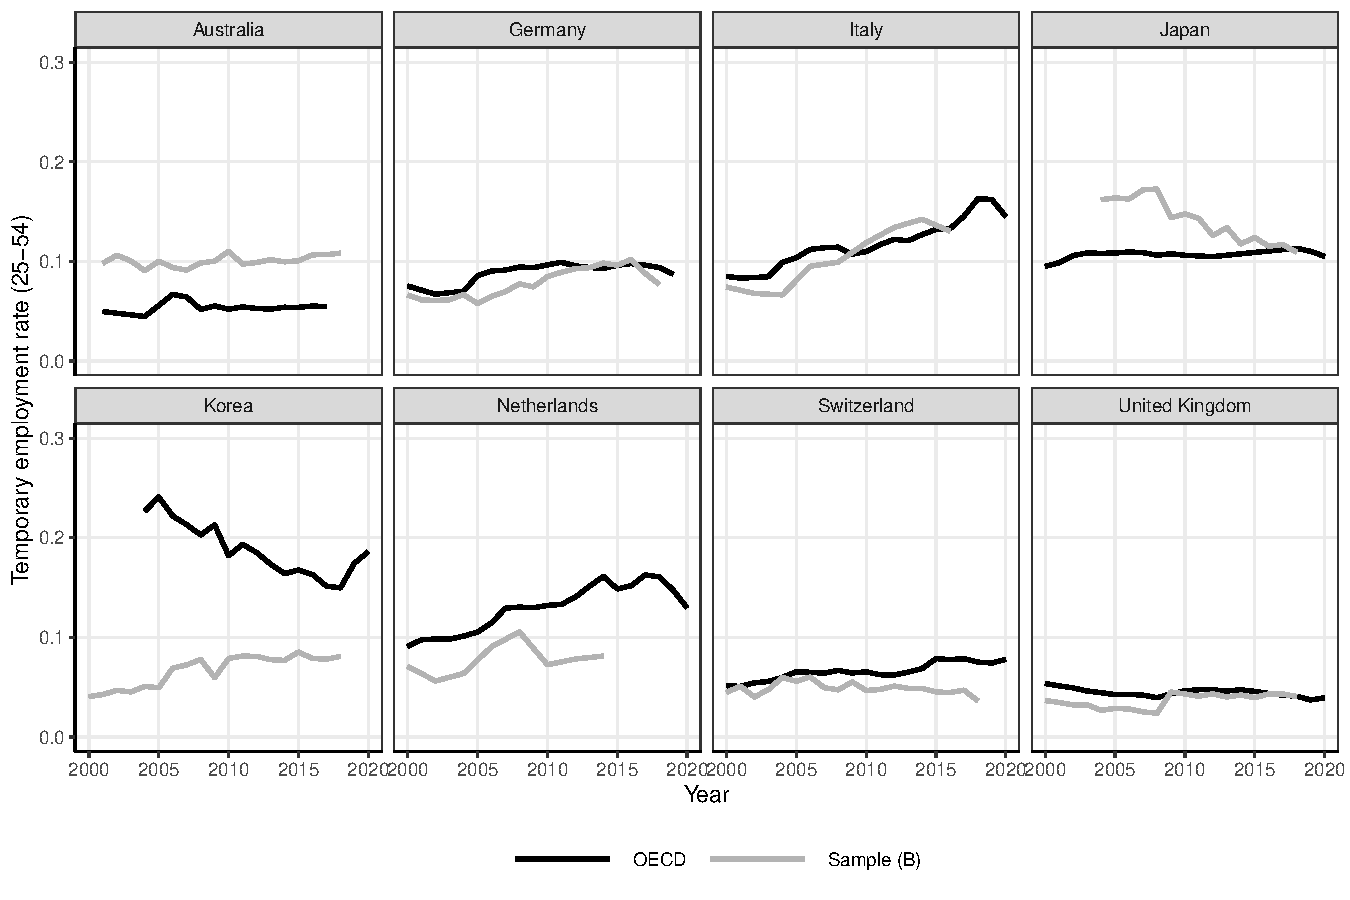
\includegraphics{../graphs/graph_descriptives_temp_paper.pdf}}
    \label{graph_descriptives_temp_paper}
\end{sidewaysfigure}

\end{document}

